\section{Testing} \label{sec:testing}

\subsection{Tecnologie usate} \label{subsec:testing-technologies}
La tecnologia utilizzata per il testing del progetto è \verb|org.scalatest| insieme a \verb|AnyFlatSpec| che permette di scrivere
test in modo semplice e  chiaro in modo che i test siano facilmente comprensibili. La libreria è inoltre supportata da IntelliJ
e permette di eseguire i test direttamente dall'IDE, rendendo il processo di testing più veloce.

\subsection{Grado di copertura} \label{subsec:testing-coverage}
Il grado di copertura dei test è del 34\%, come mostrato anche a Figura \ref{fig:coverage-report}. Analizzando meglio il report,
si può notare che, considerando solo le classi di model e di geometry, il grado di copertura sale all'88\%. Questo è dovuto al fatto
che, utlizzando un approccio TDD (Test Driven Development), e cominciando a progrmmare partendo dalle classi di model, queste sono
state testate in modo approfondito; le classi di view e controller, invece, sono state testate in modo meno approfondito perchè non
fanno altro che coordinare il sistema e visualizzare l'output, senza implementare logiche complesse. Per le classi di controller
che necessitavano di testing (es. le classi di gestione del PubSub) sono stati scritti test specifici.
\begin{figure}[h]
    \centering
    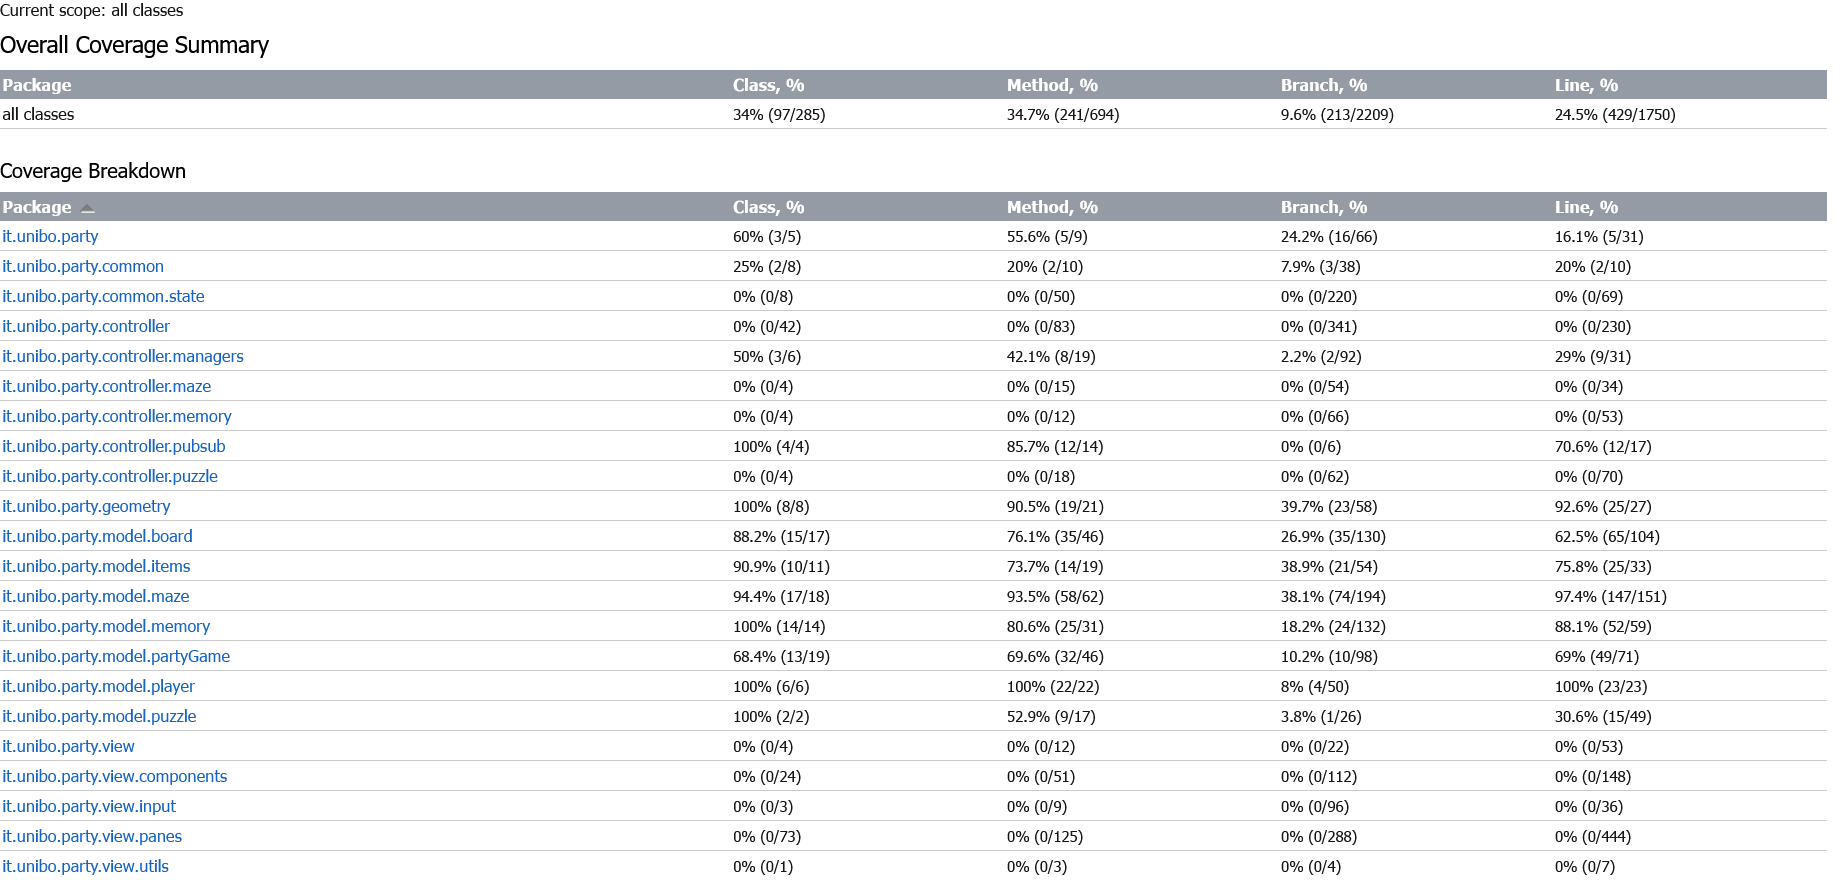
\includegraphics[width=1\textwidth]{figures/testing-coverage.png}
    \caption{Coverage report generato con IntelliJ}
    \label{fig:coverage-report}
\end{figure}

\subsection{Metodologia usata} \label{subsec:testing-methodology}
Come già accennato, il progetto è stato sviluppato utilizzando un approccio TDD (Test Driven Development), quindi i test sono stati
scritti prima della vera implementazione del codice. Come ciclo di TDD abbiamo seguito il ciclo \textit{Red-Green-Refactor} eseguendo
un commit dopo ogni completamento di un ciclo. Solo le classi di model e di utility sono state sviluppate con questo approccio, 
mentre le classi di controller hanno seguito un approccio più classico, scrivendo prima il codice e poi i test.

\subsection{Esempi rilevanti} \label{subsec:testing-examples}
Un esempio rilevante di test è quello del \verb|MazeBuilderTest| che utilizza tecniche di DSL per testare la costruizione di un 
labirinto per il minigioco maze.

\begin{lstlisting}[language=Scala]
    it should "not allow a maze that is not solvable" in:
      val builder: MazeBuilder = MazeBuilder.construct(mazeDimensions._1, mazeDimensions._2):
        W | W | E | W | W
        W | * | * | * | W
        W | * | W | W | W
        W | * | W | W | W
        W | W | X | W | W
      an[IllegalArgumentException] should be thrownBy builder.build()
\end{lstlisting}

